\documentclass[11pt]{article}
% Study guide: every mechanism of our method, step by step (purpose, procedure, mathematics).
% Build: pdflatex mechanisms.tex (twice) in docs/latex/. Contains only our method; no baselines or history.
\usepackage[a4paper,margin=2.3cm]{geometry}
\usepackage[T1]{fontenc}
\usepackage[utf8]{inputenc}
\usepackage{lmodern}
\usepackage{microtype}
\usepackage{amsmath,amssymb,amsthm,mathtools,bm}
\usepackage{booktabs,array,tabularx}
\usepackage{enumitem}
\usepackage[most]{tcolorbox}
\usepackage{tikz}
\usetikzlibrary{arrows.meta,positioning,fit}
\usepackage{xcolor}
\usepackage[hidelinks]{hyperref}
\usepackage[capitalise,nameinlink]{cleveref}

\setlist{itemsep=2pt,topsep=3pt}
\setlength{\parskip}{4pt}
\setlength{\parindent}{0pt}
\definecolor{ink}{HTML}{1F2A37}
\definecolor{blue}{HTML}{1C4E9A}
\definecolor{pale}{HTML}{EEF2F8}
\definecolor{green}{HTML}{E9F7EC}
\definecolor{amber}{HTML}{FFF4E0}

\newtcolorbox{purpose}{colback=pale,colframe=blue,boxrule=0.6pt,arc=2pt,left=6pt,right=6pt,top=4pt,bottom=4pt,
  title=Purpose,fonttitle=\bfseries\small,coltitle=white}
\newtcolorbox{steps}[1][Procedure]{colback=white,colframe=blue!60,boxrule=0.6pt,arc=2pt,left=6pt,right=6pt,
  top=4pt,bottom=4pt,title=#1,fonttitle=\bfseries\small,coltitle=white}
\newtcolorbox{keypoint}{colback=green,colframe=green!50!black,boxrule=0.6pt,arc=2pt,left=6pt,right=6pt,top=4pt,
  bottom=4pt,title=What to remember,fonttitle=\bfseries\small,coltitle=white}
\newtcolorbox{caveat}{colback=amber,colframe=orange!70!black,boxrule=0.6pt,arc=2pt,left=6pt,right=6pt,top=4pt,
  bottom=4pt,title=What it does not do,fonttitle=\bfseries\small,coltitle=white}

\theoremstyle{plain}
\newtheorem{result}{Result}
\theoremstyle{definition}
\newtheorem{example}{Worked example}

\newcommand{\E}{\mathbb{E}}
\newcommand{\R}{\mathbb{R}}
\newcommand{\norm}[1]{\lVert #1\rVert}
\newcommand{\softmax}{\operatorname{softmax}}
\newcommand{\ReLU}{\operatorname{ReLU}}
\newcommand{\LSE}{\operatorname{LSE}}
\newcommand{\KL}{\operatorname{KL}}

\title{\textbf{Our Method, Mechanism by Mechanism}\\[4pt]
\large A study guide: what each part does, how it does it, the mathematics, and why it is there}
\author{}
\date{22 October 2026}

\begin{document}
\maketitle
\vspace{-1.5em}
\setcounter{tocdepth}{1}
\tableofcontents
\newpage

% =====================================================================================================================
\section{The idea in one page}

\textbf{The setting.} $K$ clients hold private, long-tailed data: a few classes are common and many are rare, and
every client sees a different class mix. Clients run \emph{different} model architectures, so their parameters cannot
simply be averaged. Our method lives inside a three-stage pipeline (\cref{sec:skeleton}): a small shared feature
extractor, a shared generator of synthetic features, and one private model (``head'') per client.

\textbf{The problem.} Under long-tailed clients, three things go wrong. (1)~The generator forgets rare classes.
(2)~Each head's last layer is fitted to its own client's class mix. (3)~Synthetic features that do not carry their
class label actively harm the heads.

\textbf{The principle.} \emph{Wherever the data decide the answer, use a statistic that secure aggregation computes
exactly (a sum over clients) instead of a parameter that averaging only estimates.} Sums do not depend on how the
data are split across clients, so they equal what a centralised learner would compute.

\textbf{The mechanisms}, in the order they act:

\begin{center}
\small
\begin{tabularx}{\linewidth}{>{\raggedright\arraybackslash}p{3.1cm}>{\raggedright\arraybackslash}p{1.7cm}X}
\toprule
Mechanism & Stage & Problem it solves\\
\midrule
Class-statistics release (\cref{sec:release}) & after Stage I & gives the server exact class means and spreads\\
Separation $F$ and the gate (\cref{sec:gate}) & before Stage II & decides which generator can work on this data\\
Mean-anchored generator (\cref{sec:anchor}) & Stage II & removes the parameters that collapse for rare classes\\
Class rows + holder-weighted averaging (\cref{sec:hwa}) & Stage II, if $F<0.05$ & keeps class rows when means are uninformative\\
Moment correction (\cref{sec:mc}) & sampling & puts every class's samples at the exact mean and spread\\
Kernel herding, \emph{optional} (\cref{sec:kh}) & sampling & selects samples closest to the exact class fingerprint\\
Logit adjustment (\cref{sec:la}) & Stage III, real data & stops the real phase erasing what synthetic data taught\\
Consensus soft labels (\cref{sec:csl}) & Stage III, synthetic data & lowers the label error of imperfect synthetic features\\
Exact readout (\cref{sec:er}) & after Stage III & replaces each biased last layer by the centralised one\\
\bottomrule
\end{tabularx}
\end{center}

\Cref{sec:together} assembles them into one algorithm, and \cref{sec:cheatsheet} lists every symbol and setting.

% =====================================================================================================================
\section{The skeleton we build on}\label{sec:skeleton}

Only the parts of the pipeline that our mechanisms touch are described here.

\begin{center}
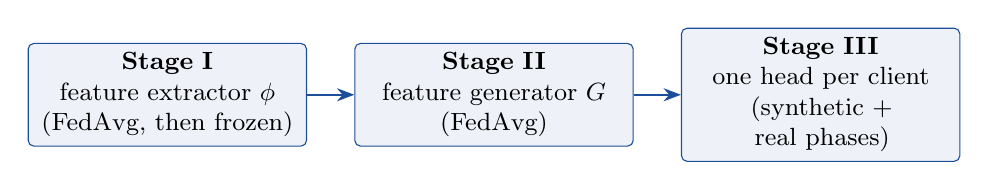
\begin{tikzpicture}[node distance=0.5cm and 0.6cm, every node/.style={font=\small},
  box/.style={draw=blue,rounded corners=2pt,fill=pale,align=center,minimum height=1.1cm,text width=3.3cm},
  arr/.style={-{Stealth[length=2.2mm]},thick,blue}]
\node[box] (s1) {\textbf{Stage I}\\feature extractor $\phi$\\(FedAvg, then frozen)};
\node[box,right=of s1] (s2) {\textbf{Stage II}\\feature generator $G$\\(FedAvg)};
\node[box,right=of s2] (s3) {\textbf{Stage III}\\one head per client\\(synthetic + real phases)};
\draw[arr] (s1) -- (s2); \draw[arr] (s2) -- (s3);
\end{tikzpicture}
\end{center}

\begin{itemize}
\item \textbf{Features.} Every image $x$ is mapped by the frozen extractor to a feature $h=\phi(x)$ (for MNIST a
$3\times16\times16$ tensor, 768 numbers; for CIFAR $10\times16\times16$). Everything after Stage I works on features.
\item \textbf{Generator.} A conditional variational autoencoder (CVAE): an encoder $q(z\mid h,y)$, a decoder that maps a
latent code $z\in\R^{16}$ (50 for CIFAR) and a class $y$ to a synthetic feature $\tilde h$. It is trained by FedAvg:
each round every client trains its copy for 5 local epochs (Adam, learning rate $10^{-3}$, weight decay $10^{-3}$) and
the server averages the copies.
\item \textbf{Heads.} Client $k$ owns a head $h_k$ of architecture $a(k)$: a \emph{body} that maps $h$ to an embedding
$e$, and a \emph{last layer} $f(e)=We+b$ giving $C$ logits. Each Stage-III round, the client trains the head for $T_s$
epochs on synthetic features and then $T_r=5$ epochs on its own real features (SGD, learning rate 0.1). Heads of the
same architecture are averaged.
\end{itemize}

\textbf{Notation.} $n_{kc}$ is client $k$'s number of class-$c$ samples, $n_c=\sum_kn_{kc}$, $N=\sum_cn_c$,
$\pi_{kc}=n_{kc}/n_k$ is client $k$'s class prior. $H_c$ is the set of $m_c$ clients that hold class $c$.

% =====================================================================================================================
\section{Foundation: why exact sums are the right tool}\label{sec:foundation}

Two short results justify every mechanism that uses sums. Read them first; the rest of the guide refers back to them.

\subsection{The client split is a pure label shift}

\begin{result}[pure label shift]\label{res:labelshift}
For every client $k$ and class $c$ with $n_{kc}>0$, client $k$'s class-$c$ samples are a uniformly random subset of
the pooled class-$c$ samples. Hence $P_k(x\mid y)=P(x\mid y)$, and, because $\phi$ is shared, $P_k(h\mid y)=P(h\mid y)$.
\end{result}

\emph{Why it holds.} The split decides \emph{how many} samples of each class a client receives, then takes them from
a random permutation of that class. A random chunk of a random permutation is a uniformly random subset.

\emph{What it buys.} Clients differ only in \emph{how much} of each class they hold, never in \emph{what} a class
looks like. So for any class-conditional quantity (a class mean, a class spread, a class row of the generator, a
readout) every client's data point at the \emph{same} target as the pooled data. Federation can cost weighting,
variance and speed, but it cannot bias such a target. A bias can only come from (i)~the optimiser, (ii)~parameters
tied to a client's own class prior (biases and last layers), or (iii)~shared parameters trained on prior-weighted
losses (equally prior-weighted centrally). The mechanisms below remove (i) and (ii).

\subsection{Sums are partition-invariant}

\begin{result}[partition invariance]\label{res:invariance}
Let a quantity be a function $\Psi(S)$ of a sum $S=\sum_{k}\sum_{i\in D_k}T(x_i,y_i)$ with $T$ fixed in advance. Its
value is the same for every way of splitting the pooled data across clients, and equals the centralised value.
\end{result}

\emph{Proof.} Addition is associative and commutative. $\square$

The result is trivial; its power is in sorting the pipeline. Anything computed from sums (class means, spreads,
fingerprints, the exact readout) is \emph{exactly} what a centralised learner would compute. Anything trained by
averaging (the generator, the bodies) is not. Our method moves as many decisions as possible into the first group.

\subsection{Secure aggregation}

Under secure aggregation each client uploads a masked vector; the masks cancel in the sum, so the server learns only
$\sum_k v_k$ and nothing about any single $v_k$. Every release in this guide is such a sum.

% =====================================================================================================================
\section{Mechanism 1: the class-statistics release}\label{sec:release}

\begin{purpose}
Give the server the exact mean and spread of every class's features, computed over all clients, without any client
revealing its own data or its own class counts.
\end{purpose}

\begin{steps}
Once, after Stage I (the extractor is frozen):
\begin{enumerate}
\item Client $k$ computes, for every class $c$: the count $n_{kc}$, the feature sum $S_{kc}=\sum_{i\in D_k,y_i=c}h_i$
(a vector), and the sum of squared norms $Q_{kc}=\sum_{i\in D_k,y_i=c}\norm{h_i}^2$ (a number).
\item Secure aggregation returns $n_c=\sum_kn_{kc}$, $S_c=\sum_kS_{kc}$, $Q_c=\sum_kQ_{kc}$.
\item The server computes the class mean and the class spread (mean squared distance to the mean):
\[
m_c=\frac{S_c}{n_c},\qquad V_c=\E\norm{h-m_c}^2=\frac{Q_c}{n_c}-\norm{m_c}^2 .
\]
\end{enumerate}
\end{steps}

\emph{Derivation of $V_c$.} $\E\norm{h-m_c}^2=\E\norm h^2-2\langle\E h,m_c\rangle+\norm{m_c}^2=\E\norm h^2-\norm{m_c}^2$,
and $\E\norm h^2=Q_c/n_c$.

\begin{example}
A class has 3 samples in total, two on client 1 and one on client 2, with (two-dimensional) features $(1,0)$, $(3,0)$
and $(2,3)$. Client 1 sends $n=2$, $S=(4,0)$, $Q=1+9=10$; client 2 sends $n=1$, $S=(2,3)$, $Q=13$. The server receives
$n=3$, $S=(6,3)$, $Q=23$, so $m=(2,1)$ and $V=23/3-5=8/3$. Computing the mean and spread directly on the three points
gives the same numbers, as \cref{res:invariance} says it must.
\end{example}

\textbf{Cost.} $C(d+2)$ numbers per client, once ($d$ = feature size). By \cref{res:labelshift,res:invariance},
$m_c$ and $V_c$ are exactly the centralised values.

\begin{caveat}
For a class with very few samples the release is close to an average over a handful of people, so it can leak
whether someone is in the data. If that matters, clip features and add Gaussian noise to the sums
(\cref{sec:privacy}).
\end{caveat}

% =====================================================================================================================
\section{Mechanism 2: the separation statistic $F$ and the gate}\label{sec:gate}

\begin{purpose}
Decide, from the released sums alone, whether class means are far enough apart to tell classes apart. If they are,
the mean-anchored generator (\cref{sec:anchor}) is used; if not, the generator keeps learned class rows protected by
holder-weighted averaging (\cref{sec:hwa}).
\end{purpose}

\textbf{Definition.} With $\bar m=\frac1C\sum_cm_c$,
\[
F=\frac{\frac1C\sum_c\norm{m_c-\bar m}^2}{\frac1C\sum_cV_c}
\quad=\quad\frac{\text{average squared distance of a class mean from the centre}}{\text{average within-class spread}} .
\]
In units of the within-class spread, two class means are on average about $\sqrt{2F}$ apart.

\textbf{Why the decision is needed.} The mean-anchored generator receives a class only through its mean $m_y$. If two
classes have nearly the same mean, it cannot produce different samples for them:

\begin{result}[what a mean anchor can express]\label{res:w1}
Let the class-$c$ sampler be $X_c=\ReLU(m_c+g(Z,Am_c))$, with the noise $Z$ shared by all classes, $A$ a class-shared
matrix and $g$ $L$-Lipschitz in its second argument. Then for any two classes
\[
W_1(G_c,G_{c'})\le(1+L\norm{A}_2)\,\norm{m_c-m_{c'}} .
\]
\end{result}
\emph{Proof.} Use the same $Z$ for both classes. ReLU is 1-Lipschitz, so
$\norm{X_c-X_{c'}}\le\norm{m_c-m_{c'}}+\norm{g(Z,Am_c)-g(Z,Am_{c'})}\le(1+L\norm A_2)\norm{m_c-m_{c'}}$; take
expectations. $\square$

($W_1$ is the earth-mover distance: the average distance samples must move to turn one class's distribution into
the other's.) If $\norm{m_c-m_{c'}}$ is tiny relative to the spread, the synthetic classes are nearly identical, and no
amount of training changes that.

\begin{steps}[Decision rule]
Compute $F$ from the released sums. If $F\ge0.05$: use the mean-anchored generator. If $F<0.05$: use class rows with
holder-weighted averaging.
\end{steps}

\textbf{Measured values.} $F$ is 0.25 or more on MNIST and FashionMNIST, 0.18--0.25 on CIFAR-100, 0.054--0.080 on
CIFAR-10, and 0.005--0.013 on SVHN. So the gate chooses class rows only on SVHN, where class means differ by just
10--15\% of the within-class spread.

\begin{caveat}
The threshold 0.05 was set after seeing SVHN; CIFAR-10 is close to it. On CIFAR-10 both branches were run and give
the same accuracy (within 0.13 points), so the choice did not matter there.
\end{caveat}

% =====================================================================================================================
\section{Mechanism 3: the mean-anchored generator}\label{sec:anchor}

\begin{purpose}
Remove the only parameters through which a FedAvg-trained generator forgets rare classes, by giving the generator the
exact class mean instead of a learned class row.
\end{purpose}

\subsection{The failure it removes}

In a standard conditional generator, class $c$ enters through a learned row $r_c\in\R^{512}$ (a column of the label
projection). It is the only class-specific parameter, and its data gradient is non-zero only on samples of class $c$.

Consider one round. Client $k$ starts from the global row $r_c$, trains locally and returns $r_{k,c}$. Write
$\Delta_k=\norm{r_{k,c}}-\norm{r_c}$, the holders' mean gain $\bar G_c=\frac1{m_c}\sum_{k\in H_c}\Delta_k$ and the
non-holders' mean loss $\bar D_c=-\frac1{K-m_c}\sum_{k\notin H_c}\Delta_k$, with $p_c=m_c/K$.

\begin{result}[contraction bound]\label{res:contraction}
With plain averaging $r_c^+=\frac1K\sum_kr_{k,c}$:
\[
\norm{r_c^+}\le\norm{r_c}+p_c\bar G_c-(1-p_c)\bar D_c .
\]
\end{result}
\emph{Proof.} Triangle inequality: $\norm{\frac1K\sum_kr_{k,c}}\le\frac1K\sum_k\norm{r_{k,c}}=\norm{r_c}+\frac1K\sum_k\Delta_k$;
split the sum into holders ($m_c\bar G_c$) and non-holders ($-(K-m_c)\bar D_c$). $\square$

\textbf{Why non-holders shrink the row fast: Adam with coupled decay.} A client without class $c$ has zero data
gradient on $r_c$, so its gradient is pure weight decay, $\lambda r_c$. Adam divides each gradient by the root of its
own running average of squares, $\hat m/\sqrt{\hat v}$, so it is (almost) blind to the size of the gradient: a gradient
of $\lambda r_c$ produces a step of about the learning rate $\eta$ toward zero, \emph{whatever} $\lambda$ is. Holders,
meanwhile, use $r_c$ to fit their data, which does not push its norm up at full speed. So $\bar D_c\gg\bar G_c$ and the
right-hand side of \cref{res:contraction} is negative even when most clients hold the class. Measured on MNIST, where
every class is held by at least 7 of 10 clients, the three rarest classes' rows shrank to 4--10\% of their initial
length.

\textbf{A rule from counts alone.} Per coordinate an Adam step is $\eta\psi$ with $\psi\in[-1,1]$. A non-holder
takes $\tau_k$ steps of size $\eta$ toward zero; a holder moves the row only on its $\tau_kf_{kc}$ steps whose batch
contains $c$ ($f_{kc}$ = probability that a batch of client $k$ contains class $c$). Hence the ratio
\[
\kappa_c=\frac{\sum_{k\in H_c}\tau_kf_{kc}}{\sum_{k\notin H_c}\tau_k}
\]
of ``steps that can grow the row'' to ``steps that shrink it''. If $\kappa_c<1$ the averaged drift points to zero for
every coordinate: the row collapses. Across 900 logged rows, all 352 rows with $\kappa_c<1$ collapsed, and a prediction
written down before new runs held for 16 of 16 rows.

\subsection{How the mean anchor works}

\begin{steps}[Architecture (PC-VAE)]
\begin{enumerate}
\item \textbf{Anchor.} The exact class means $m_c$ of \cref{sec:release} are stored inside the generator as fixed
buffers (not trained).
\item \textbf{Encoder.} It sees the real feature and its class mean stacked as channels, $[h,m_y]$, and outputs the
mean and log-variance of $q(z\mid h,y)$.
\item \textbf{Decoder.} It forms $a=W_zz+Pm_y$ with a class-\emph{shared} projection $P$, and outputs only the
deviation from the class mean:
\[
\tilde h=\ReLU\big(m_y+\mathrm{dec}(\ReLU(a))\big).
\]
\item \textbf{Loss.} The usual evidence lower bound: reconstruction error plus $\KL(q(z\mid h,y)\,\|\,\mathcal N(0,I))$.
\item \textbf{Training.} FedAvg exactly as before (same optimiser, same rounds).
\item \textbf{Sampling.} Draw $z\sim\mathcal N(0,I)$ and decode with the requested class $y$.
\end{enumerate}
\end{steps}

\textbf{Why this removes the collapse.} No parameter is specific to a class: $W_z$, $P$ and the decoder are shared by
all classes and receive gradients from every client. So non-holders have nothing class-specific to shrink, and
\cref{res:contraction} has nothing to act on. Rare classes also borrow the \emph{shape} of within-class variation from
all classes through the shared decoder, while their location comes from their exact mean. (If the decoder were
linear, this would be a Gaussian model with exact class means.)

\begin{caveat}
The anchor does not force samples to carry their class: when class means are close, the decoder can ignore $m_y$
(\cref{res:w1}). That is why the gate exists.
\end{caveat}

% =====================================================================================================================
\section{Mechanism 4: class rows with holder-weighted averaging}\label{sec:hwa}

\begin{purpose}
On data where class means are nearly identical ($F<0.05$), keep the generator's learned class rows, which can encode
differences the means cannot, but stop them from collapsing.
\end{purpose}

\begin{steps}
The generator is the standard one with class rows $r_c$. All parameters except the rows are averaged by FedAvg. Each
row is averaged only over clients that hold the class, weighted by their effective number of samples:
\[
r_c\leftarrow\frac{\sum_kE(n_{kc})\,r_{k,c}}{\sum_kE(n_{kc})},\qquad E(n)=\frac{1-\beta^{\,n}}{1-\beta},\quad\beta=0.999 .
\]
\end{steps}

\textbf{What it does.} Non-holders have $E(0)=0$, so their decay-only copies are excluded. By the triangle inequality
\(\norm{r_c^+}\le\norm{r_c}+\sum_{k\in H_c}\omega_k\Delta_k\) with $\omega_k\propto E(n_{kc})$: the $-(1-p_c)\bar D_c$ term
of \cref{res:contraction} disappears. HWA does not force a row to grow; it leaves it to the holders.

\textbf{Why weight by $E(n)$.} $E(n)$ grows like $n$ for small $n$ and saturates for large $n$ (at most
$1/(1-\beta)=1000$). It interpolates between weighting holders by their counts ($\beta\to1$) and weighting them equally
($\beta\to0$). What matters most is excluding non-holders; the exact weights change little.

\textbf{It also fixes a slower problem.} Even without decay, plain averaging dilutes a rare row's learning rate by
$m_c/K$ (non-holders contribute no movement but still count in the average), and in the limit of long local training
it averages the holders' local means \emph{unweighted}:

\begin{result}[dilution under plain averaging; quadratic row model]\label{res:dilution}
If each holder's local training converges to its local class mean $\bar t_{kc}$, plain averaging converges to the
unweighted mean of the $\bar t_{kc}$, whose mean squared error is
\[
V_c=\frac{n_c}{m_c^2}\sum_{k\in H_c}\frac1{n_{kc}}\ \ge\ 1
\]
times that of the pooled mean (equality iff all holders have equal counts), and it gets there $m_c/K$ times more
slowly. With weights $E(n_{kc})\approx n_{kc}$, HWA gives $V_c\approx1$ and no dilution.
\end{result}
\emph{Proof sketch.} Non-holders map the row to itself and drop out of the fixed point. The unweighted mean of
independent unbiased local means (\cref{res:labelshift}) has variance $\frac1{m_c^2}\sum_k\sigma^2/n_{kc}$, against
$\sigma^2/n_c$ for the pooled mean. $\square$

\textbf{Privacy.} The server needs only $\sum_kE(n_{kc})r_{k,c}$ and $\sum_kE(n_{kc})$, two sums, so HWA runs under
secure aggregation and reveals neither any client's row nor its class counts. When all clients have equal counts,
HWA is exactly FedAvg.

% =====================================================================================================================
\section{Mechanism 5: moment correction}\label{sec:mc}

\begin{purpose}
Generators trained by maximum likelihood tend to produce samples that are too concentrated and, for rare classes,
centred in the wrong place. Moment correction moves each class's synthetic samples so that their mean and spread equal
the exact class mean $m_c$ and spread $V_c$, while changing them as little as possible.
\end{purpose}

\begin{steps}
Once, after Stage II:
\begin{enumerate}
\item For each class $c$, draw 500 samples from the generator and measure their mean $\tilde m_c$ and spread
$\tilde V_c=\E\norm{\tilde h-\tilde m_c}^2$.
\item Compute the scale $s_c=\sqrt{V_c/\tilde V_c}$, clipped to $[0.1,10]$ for safety.
\end{enumerate}
Every time a class-$c$ sample $x$ is drawn afterwards:
\[
x'=\ReLU\big(m_c+s_c\,(x-\tilde m_c)\big).
\]
\end{steps}

\textbf{The mathematics: the smallest change with the right moments.}

\begin{result}[minimum-displacement correction]\label{res:mc}
Let $X$ have mean $\tilde m$ and spread $\tilde V$. Among \emph{all} maps $T$ with $\E\,T(X)=m$ and
$\E\norm{T(X)-m}^2=V$, the map $T^\star(x)=m+\sqrt{V/\tilde V}\,(x-\tilde m)$ minimises the average displacement
$\E\norm{T(X)-X}^2$.
\end{result}
\emph{Proof.} Let $Y=T(X)$. Expanding around the two means,
\[
\E\norm{Y-X}^2=V+\tilde V+\norm{m-\tilde m}^2-2\,\E\langle Y-m,\;X-\tilde m\rangle .
\]
Only the last term depends on how $Y$ is coupled to $X$. By Cauchy--Schwarz,
$\E\langle Y-m,X-\tilde m\rangle\le\sqrt{\E\norm{Y-m}^2\,\E\norm{X-\tilde m}^2}=\sqrt{V\tilde V}$, with equality exactly
when $Y-m$ is a positive multiple of $X-\tilde m$, i.e.\ $Y-m=\sqrt{V/\tilde V}(X-\tilde m)$. $\square$

\textbf{Reading.} The correction shifts the cloud of samples to the right centre and stretches or shrinks it to the
right size, but keeps its \emph{shape}: the directions of variation the generator learned are preserved. It needs no
new release: $m_c$ and $V_c$ come from \cref{sec:release}.

\begin{example}
For a rare class the generator's samples have mean $\tilde m=(1,1)$ and spread $\tilde V=0.5$, while the exact
statistics are $m=(2,1)$ and $V=2$. Then $s=\sqrt{2/0.5}=2$, and a sample $x=(1.5,0.5)$ becomes
$(2,1)+2\,(0.5,-0.5)=(3,0)$: the cloud moves one unit to the right and doubles its radius.
\end{example}

\begin{caveat}
After the final ReLU (features are non-negative) and with moments estimated from 500 samples, the corrected
moments match only approximately. Moment correction cannot create class differences that the generator does not
produce; it only fixes location and scale.
\end{caveat}

% =====================================================================================================================
\section{Mechanism 6 (optional): kernel herding}\label{sec:kh}

\begin{purpose}
Choose, among many synthetic samples of a class, the subset whose overall distribution is closest to the real class's,
as measured by a kernel ``fingerprint'' that the server can compute exactly.
\end{purpose}

\textbf{The fingerprint.} Random Fourier features turn a feature $h$ into a vector
\[
\varphi(h)=\sqrt{2/D}\,\cos(\Omega h+b)\in\R^{D},\qquad D=6144,
\]
with the rows of $\Omega$ drawn from Gaussians of three widths ($s_0\times\{0.5,1,2\}$, $s_0=\sqrt{2\,\overline{V_c}}$)
and $b$ uniform on $[0,2\pi]$. Inner products approximate a Gaussian kernel,
$\langle\varphi(h),\varphi(h')\rangle\approx k(h,h')$, and $\norm{\varphi(h)}\le\sqrt2$. A class's fingerprint is the
average $\mu_c=\frac1{n_c}\sum_{i:y_i=c}\varphi(h_i)$, released as a sum $\sum_i\varphi(h_i)$ like the other statistics.
The distance between two fingerprints is the maximum mean discrepancy (MMD) between the two distributions.

\begin{steps}
For each class $c$, when $n$ samples are needed:
\begin{enumerate}
\item Draw $4n$ moment-corrected candidates and compute their fingerprints $\varphi_1,\dots,\varphi_{4n}$.
\item Greedily pick $n$ of them without replacement. With $w_0=\mu_c$, at step $t$ pick
$j_t=\arg\max_i\langle\varphi_i,w_t\rangle$ among unpicked candidates, then update $w_{t+1}=w_t+\mu_c-\varphi_{j_t}$.
\end{enumerate}
\end{steps}

\emph{Why this rule.} After $t$ picks, $w_t=(t+1)\mu_c-\sum_{s\le t}\varphi_{j_s}$, which points from the current
selection's average toward the target fingerprint. Picking the candidate most aligned with it is the step that most
reduces $\norm{\frac1t\sum_s\varphi_{j_s}-\mu_c}$, the MMD between the selection and the real class.

\textbf{Motivation.} If a head's loss $\ell$ lies in the kernel's function space with norm at most $B$, then
$|\E_{\text{synthetic}}\ell-\E_{\text{real}}\ell|\le B\cdot\mathrm{MMD}$. ReLU networks do not satisfy this premise, so
this is a motivation, not a guarantee.

\begin{keypoint}
Kernel herding is consistently positive but small: removing it costs $0.1$--$0.4$ points with the exact readout
(positive in 8 of 8 paired seeds), while it makes the head stage about $6\times$ slower. A larger fingerprint or
candidate pool changes nothing. It is therefore \textbf{optional}: being closer in distribution is not the same as
being more useful to the classifier.
\end{keypoint}

% =====================================================================================================================
\section{Mechanism 7: logit adjustment in the real phase}\label{sec:la}

\begin{purpose}
Train each head on its own real data in a way that targets \emph{balanced} accuracy, and, crucially, stop the real
phase from erasing what the synthetic phase taught the head about classes this client does not have.
\end{purpose}

\begin{steps}
Client $k$ estimates its class prior with add-one smoothing, $\hat\pi_{kc}=(n_{kc}+1)/(n_k+C)$, which never leaves
the client. In the real phase it minimises
\[
\ell_{\mathrm{LA}}(h,y)=-\log\frac{\exp\big(f_y(h)+\tau\log\hat\pi_{ky}\big)}{\sum_j\exp\big(f_j(h)+\tau\log\hat\pi_{kj}\big)},
\qquad\tau=1 .
\]
At test time the plain logits $f(h)$ are used. The synthetic phase uses unadjusted logits.
\end{steps}

\textbf{Why it targets balanced accuracy.} Bayes' rule gives $\log p_k(y\mid h)=\log p(h\mid y)+\log\pi_{ky}+\text{const}$,
and $p(h\mid y)$ is the same for every client (\cref{res:labelshift}). Training $f+\log\hat\pi_k$ to match the client's
posterior makes $f$ match $\log p(h\mid y)$, the prior-free score, whose arg-max is the balanced-error-optimal decision.

\textbf{What it cannot do on its own.}

\begin{result}[logit corrections are reparametrisations]\label{res:reparam}
For a head with a free last-layer bias $b$ trained by SGD, training with $\ell(f+a_k,y)$ from $(\theta_0,b_0)$, for any
fixed vector $a_k$, gives exactly the same trajectory as training with $\ell(f,y)$ from $(\theta_0,b_0+a_k)$: every
parameter except $b$ is identical at every step, and $b^{\mathrm{LA}}_t=b^{\mathrm{CE}}_t-a_k$.
\end{result}
\emph{Proof.} $f+a_k=We+(b+a_k)$, and $b\mapsto b+a_k$ is a translation with identity Jacobian, so the gradients at
corresponding points agree; induct over steps. $\square$

So for a head trained on real data alone, logit adjustment changes only the bias: it is a readout correction, and the
exact readout (\cref{sec:er}) makes it redundant there. Its real job is during training, because of how the two phases
alternate:

\begin{result}[what the alternation keeps; quadratic losses]\label{res:alternation}
Let the synthetic and real losses be quadratic with Hessians $H_s,H_r$ and minimisers $\theta_s,\theta_r$, and let each
round take $S_s$ synthetic then $S_r$ real gradient steps, $P_s=(I-\eta H_s)^{S_s}$, $P_r=(I-\eta H_r)^{S_r}$. The rounds
converge to
\[
\theta^\star=\theta_r+\Omega(\theta_s-\theta_r),\qquad\Omega=(I-P_rP_s)^{-1}P_r(I-P_s).
\]
Along an eigendirection $i$ (commuting Hessians) the weight of the synthetic solution is
$\omega_i=\frac{\rho_{r,i}(1-\rho_{s,i})}{1-\rho_{r,i}\rho_{s,i}}\le\rho_{r,i}=(1-\eta h_{r,i})^{S_r}$.
\end{result}
\emph{Proof.} A round is the affine map $\theta\mapsto P_rP_s\theta+P_r(I-P_s)\theta_s+(I-P_r)\theta_r$; solve for its
fixed point. $\square$

\textbf{Reading.} Where the real loss is flat ($h_{r,i}=0$, so $\rho_{r,i}=1$), the synthetic phase decides
($\omega_i=1$); where the real loss is curved, the real phase overwrites it. The flat directions are exactly those of
classes the client lacks, which are the ones balanced accuracy needs. But with plain cross-entropy the real loss is
\emph{not} flat there: it keeps pushing the logits of absent classes down without limit (as on separable data), so the
real phase erases what the synthetic phase put in. With logit adjustment, absent classes have tiny adjusted
probability ($\log\hat\pi_{kc}$ very negative), their gradient is $O(1/(n_k+C))$, and the synthetic knowledge
survives. Measured: the share of the synthetic phase's change to absent-class rows that survives the next real phase is
0.96--1.0 with logit adjustment and 0.76--0.98 without.

% =====================================================================================================================
\section{Mechanism 8: consensus soft labels on synthetic features}\label{sec:csl}

\begin{purpose}
Give each synthetic feature a target that reflects what it actually looks like, not only the class it was generated
for, so that imperfect synthetic features teach less wrong information.
\end{purpose}

\subsection{Why synthetic labels matter: the signal fraction}

\begin{result}[label-free synthetic data penalise the spread of the logits]\label{res:logitvar}
If a synthetic feature's label $y$ is uniform on the $C$ classes and independent of the feature, then for every logit
vector $f$, with $\bar f=\frac1C\sum_cf_c$,
\[
\E_y\,\ell(f,y)=\LSE(f)-\bar f=\log C+\KL\big(u\,\|\,\softmax f\big)=\log C+\frac1{2C}\sum_c(f_c-\bar f)^2+O(\norm{f-\bar f}^3).
\]
\end{result}
\emph{Proof.} Cross-entropy is $\LSE(f)-f_y$; averaging over a uniform $y$ gives $\LSE(f)-\bar f$. The KL divergence
from the uniform distribution $u$ to $\softmax f$ is $-\log C+\LSE(f)-\bar f$. Expand $\LSE$ around equal logits for the
quadratic term. $\square$

\textbf{Reading.} Synthetic features that carry no class information do not teach nothing: they teach the head to make
all logits equal on them, i.e.\ to be unsure, exactly in the region where the real data are (the generator was fitted
to them). If a fraction $s$ of synthetic features carries its label (the \emph{signal fraction}) and the rest do not,
the synthetic loss is $s\cdot(\text{useful cross-entropy})+(1-s)\cdot(\text{penalty above})$. So the synthetic phase
helps when $s$ is high and harms when $s\approx0$; measured, the gain changes sign between $s\approx0.03$ and $0.07$.
The anchor and moment correction raise $s$; consensus labels lower the damage of the part that remains wrong.

\subsection{How consensus labels work}

\begin{steps}
Every Stage-III round:
\begin{enumerate}
\item The server draws one shared pool of synthetic features $\tilde h$ with uniformly random classes $y$ (from a public
seed, so clients can regenerate it).
\item Each architecture's current head $h_g$ evaluates the pool; the server averages their probabilities (a sum over
architectures, so it fits secure aggregation):
\[
\bar p(\tilde h)=\frac1G\sum_{g=1}^{G}\softmax h_g(\tilde h).
\]
\item The target for each synthetic feature is
\[
t(\tilde h)=(1-\beta)\,e_y+\beta\,\bar p(\tilde h),\qquad\beta=0.5,
\]
where $e_y$ is the one-hot vector of its generated class.
\item Each client trains its head for $T_s$ epochs on its slice of the pool with the soft cross-entropy
$-\sum_ct_c(\tilde h)\log\softmax_c f(\tilde h)$.
\end{enumerate}
\end{steps}

\textbf{Why mix, and why $\beta=\tfrac12$.} The best possible target for a feature is its true posterior
$p(\cdot\mid\tilde h)$; the one-hot label is off by the generator's error. The ensemble of $G$ heads of different
architectures, trained on different clients, approximates that posterior with errors that partly cancel (variance down
by up to $1/G$). Keeping half of the one-hot label bounds the damage if the ensemble shares an error. A stylised model
makes the trade-off explicit:

\begin{result}[label error limits the useful amount of synthetic data]\label{res:budget}
A head estimates a parameter from $n_r$ real samples (variance $\sigma^2$ each) and a fraction $\lambda$ of $n_s$
synthetic samples whose labels have bias $b$. Writing $w=\frac{\lambda n_s}{n_r+\lambda n_s}$, the mean squared error is
$\mathcal E(w)=\frac{\sigma^2(1-w)}{n_r}+w^2b^2$, minimised at $w^\star=\frac{\sigma^2}{2n_rb^2}$ (clipped to the
feasible range). The optimal synthetic share falls as the label bias $b$ grows, and reaches all available synthetic
data as $b\to0$.
\end{result}
\emph{Proof.} $\mathcal E$ is a convex parabola in $w$; set its derivative to zero. $\square$

\textbf{Reading.} With hard labels, more synthetic epochs eventually hurt, because the label bias does not average
away. Moving the target toward the posterior lowers $b$, so the same synthetic budget becomes useful. This is why
consensus labels and a larger $T_s$ work together.

\textbf{Cost.} The server broadcasts the pool seed and $P\times C$ soft labels per round (about 24\,KB here). No real
data are used.

% =====================================================================================================================
\section{Mechanism 9: the exact readout}\label{sec:er}

\begin{purpose}
Replace each architecture's last layer, which is biased toward its own clients' class mix, by the class-balanced linear
classifier computed from exact sums over \emph{all} clients. This removes the single largest loss.
\end{purpose}

\textbf{Where the formula comes from.} Suppose that, in the embedding space $e=\mathrm{body}(h)$ of one architecture,
each class is Gaussian with its own mean $\mu_c$ and a shared covariance $\Sigma$, and that we want to treat all classes
as equally likely (balanced accuracy). Then
\[
\log p(e\mid c)=-\tfrac12(e-\mu_c)^\top\Sigma^{-1}(e-\mu_c)+\text{const}
=\mu_c^\top\Sigma^{-1}e-\tfrac12\mu_c^\top\Sigma^{-1}\mu_c+(\text{terms without }c),
\]
which is linear in $e$: a last layer with $w_c=\Sigma^{-1}\mu_c$ and $b_c=-\frac12\mu_c^\top\Sigma^{-1}\mu_c$. This is
linear discriminant analysis with a uniform class prior.

\begin{steps}
Once, after Stage III, for each architecture $g$:
\begin{enumerate}
\item The server broadcasts the body of architecture $g$ to every client (bodies are small).
\item Each client embeds its real features, $e=\mathrm{body}_g(h)$, and uploads per-class counts $n_c$, per-class sums
$\sum e$ and the total second moment $M=\sum ee^\top$.
\item The server computes class means $\mu_c$ and the pooled within-class covariance
\[
S=\frac{M-\sum_cn_c\mu_c\mu_c^\top}{N-C},
\]
shrinks it toward a multiple of the identity for stability,
\[
S_\gamma=(1-\gamma)S+\gamma\,\frac{\operatorname{tr}S}{d}\,I,\qquad\gamma=0.1,
\]
and sets the last layer to $w_c=S_\gamma^{-1}\mu_c$, $b_c=-\frac12\mu_c^\top S_\gamma^{-1}\mu_c$.
\end{enumerate}
\end{steps}

\emph{Derivation of $S$.} $\sum_c\sum_{i\in c}(e_i-\mu_c)(e_i-\mu_c)^\top=\sum_ie_ie_i^\top-\sum_cn_c\mu_c\mu_c^\top$,
divided by the degrees of freedom $N-C$.

\textbf{Why it is exact.} Everything the server uses is a sum, so by \cref{res:invariance} the readout equals the one a
centralised learner would compute for the same bodies. The federated last layer then stops being a source of loss
relative to centralised training. It never uses the trained last layer, so its accuracy is a direct measure of how well
the \emph{body} separates the classes. It also makes logit adjustment's bias correction redundant (\cref{res:reparam}),
but not its training role (\cref{res:alternation}).

\textbf{Cost.} One extra round; per client, up to about $5\times10^5$ numbers per architecture (the symmetric $d\times d$
second moment for $d\le1024$).

\begin{caveat}
It is only as good as the body: it removes the last-layer loss, not the representation's. The linear-Gaussian model is
an approximation; shrinkage keeps it stable for rare classes.
\end{caveat}

% =====================================================================================================================
\section{Optional: noise on the released sums}\label{sec:privacy}

\begin{purpose}
Bound what the released class statistics reveal about any individual sample, at a known cost in accuracy.
\end{purpose}

Each feature is clipped to norm at most $c_{\max}$, $h\mapsto h\min(1,c_{\max}/\norm h)$, so one sample changes $n_c$ by
1, $S_c$ by at most $c_{\max}$, $Q_c$ by at most $c_{\max}^2$ and the fingerprint sum by at most $\sqrt2$. Gaussian noise
$\sigma\times$(that sensitivity) is added to each release, with $\sigma=\sqrt{2/\rho}$ and the privacy budget
$\rho=\big(\sqrt{\log(1/\delta)+\varepsilon}-\sqrt{\log(1/\delta)}\big)^2$ (zero-concentrated differential privacy, split
equally over the releases). A class whose noisy statistic is too noisy relative to its size simply skips moment
correction and herding. The guarantee covers the added statistics only, not the FedAvg training of the generator or
heads.

% =====================================================================================================================
\section{Putting it together}\label{sec:together}

\begin{steps}[The full algorithm]
\begin{enumerate}[leftmargin=1.4em]
\item \textbf{Stage I.} Train the feature extractor $\phi$ by FedAvg; freeze it.
\item \textbf{Release} (\cref{sec:release}). Secure-aggregate $n_c$, $\sum h$, $\sum\norm h^2$ per class (and $\sum\varphi(h)$ if
herding is used). Server: $m_c$, $V_c$, $F$ (and $\mu_c$).
\item \textbf{Gate} (\cref{sec:gate}). If $F\ge0.05$, build the mean-anchored generator with the $m_c$ as buffers;
else the class-row generator.
\item \textbf{Stage II} (\cref{sec:anchor,sec:hwa}). Train the generator by FedAvg; with class rows, average each row by
HWA.
\item \textbf{Sampler} (\cref{sec:mc,sec:kh}). Measure $\tilde m_c$, $\tilde V_c$ from 500 samples per class; from now on
every sample is moment-corrected (and, optionally, herded).
\item \textbf{Stage III}, for each round:
  \begin{enumerate}
  \item Server: draw the shared synthetic pool; collect every architecture's probabilities on it; form consensus
  targets $t=\frac12e_y+\frac12\bar p$ (\cref{sec:csl}).
  \item Each client: $T_s$ epochs on its slice of the pool with soft cross-entropy; then $T_r=5$ epochs on its real
  features with logit adjustment by its own prior (\cref{sec:la}).
  \item Server: average heads within each architecture.
  \end{enumerate}
\item \textbf{Exact readout} (\cref{sec:er}). For each architecture, secure-aggregate $n_c$, $\sum e$, $\sum ee^\top$ of its
embeddings over all clients; replace the last layer by $S_\gamma^{-1}\mu_c$, $-\frac12\mu_c^\top S_\gamma^{-1}\mu_c$.
\end{enumerate}
\end{steps}

\textbf{What each problem meets.}
\begin{center}
\small
\begin{tabularx}{\linewidth}{>{\raggedright\arraybackslash}p{4.2cm}X}
\toprule
Problem & Mechanisms that address it\\
\midrule
Rare classes collapse in the generator & mean anchor (no class rows); HWA when rows are needed\\
Rare-class samples in the wrong place or too narrow & moment correction (exact mean and spread)\\
Classes the generator cannot separate & gate on $F$, falling back to class rows\\
Synthetic features with wrong labels & consensus soft labels; higher signal fraction from anchor + correction\\
Real phase erases knowledge of absent classes & logit adjustment by the client's own prior\\
Last layer fitted to one client's class mix & exact readout from sums over all clients\\
\bottomrule
\end{tabularx}
\end{center}

\textbf{What travels, and when.}
\begin{center}
\small
\begin{tabularx}{\linewidth}{>{\raggedright\arraybackslash}p{3.6cm}>{\raggedright\arraybackslash}p{3cm}X}
\toprule
Message & When & Content\\
\midrule
Class statistics & once, after Stage I & $C(d+2)$ numbers per client (plus $CD$ for herding), summed\\
HWA sums & each Stage-II round (rows only) & $\sum_kE(n_{kc})r_{k,c}$ and $\sum_kE(n_{kc})$\\
Consensus probabilities & each Stage-III round & $P\times C$ per architecture, summed\\
Exact-readout sums & once, at the end & $n_c$, $\sum e$, $\sum ee^\top$ per architecture\\
\bottomrule
\end{tabularx}
\end{center}
No raw image, real feature, label or single-client statistic ever leaves a client.

% =====================================================================================================================
\section{Cheat sheet}\label{sec:cheatsheet}

\begin{center}
\small
\begin{tabularx}{\linewidth}{>{\raggedright\arraybackslash}p{2.6cm}X}
\toprule
Symbol & Meaning\\
\midrule
$h=\phi(x)$ & feature of an image from the frozen extractor\\
$n_{kc},\ n_c,\ N$ & class-$c$ count on client $k$, over all clients, total\\
$\hat\pi_{kc}$ & client $k$'s smoothed class prior, $(n_{kc}+1)/(n_k+C)$\\
$m_c,\ V_c$ & exact class mean and spread of features\\
$F$ & class separation: mean squared distance of class means from their centre over mean spread\\
$r_c$ & class row of the class-row generator\\
$H_c,\ m_c$ (count) & clients holding class $c$, and their number\\
$\kappa_c$ & steps that can grow row $c$ over steps that shrink it; $<1$ means collapse\\
$E(n)$ & effective number of samples, $(1-\beta^n)/(1-\beta)$\\
$\tilde m_c,\ \tilde V_c,\ s_c$ & generator's class mean and spread; correction scale $\sqrt{V_c/\tilde V_c}$\\
$\varphi,\ \mu_c$ & random-feature map and exact class fingerprint (herding only)\\
$s$ & signal fraction: share of synthetic features that carry their label\\
$\bar p(\tilde h),\ t(\tilde h)$ & averaged head probabilities; consensus target\\
$e,\ \mu_c,\ S_\gamma$ & embedding of a head's body; its class mean; shrunk within-class covariance\\
\bottomrule
\end{tabularx}
\end{center}

\begin{center}
\small
\begin{tabularx}{\linewidth}{>{\raggedright\arraybackslash}p{4.6cm}X}
\toprule
Setting & Value\\
\midrule
Gate threshold on $F$ & 0.05\\
Generator latent size & 16 (50 on CIFAR)\\
Generator training & 5 local epochs per round, Adam, learning rate $10^{-3}$, weight decay $10^{-3}$\\
HWA & $\beta=0.999$\\
Moment correction & 500 samples per class; scale clipped to $[0.1,10]$\\
Kernel herding (optional) & $4\times$ candidates; $D=6144$ random features, three widths\\
Logit adjustment & $\tau=1$, add-one smoothed client prior\\
Consensus labels & $\beta=0.5$; one shared pool per round\\
Stage-III epochs & $T_s$ synthetic (chosen on validation data; 10 or 1), $T_r=5$ real; SGD, learning rate 0.1\\
Exact readout & shrinkage $\gamma=0.1$\\
\bottomrule
\end{tabularx}
\end{center}

\end{document}
